% Capítulo 2
\chapter{Capítulo 2}

Neste capítulo, descrevemos o funcionamento do sistema \texttt{Glycan RegEx}
implementado no módulo \texttt{glycowork.motif.regex}, suas funções principais,
o papel das expressões regulares e as vantagens do uso desse sistema.

O \texttt{Glycan RegEx}, introduzido por Bennett e Bojar (2024) no pacote
\texttt{glycowork}, representa um avanço significativo na análise computacional
de glicanos ao acrescentar o uso de RegEx para identificação e extração de
motifs. Tal sistema foi proposto como uma adaptação das tradicionais RegEx de
ciência da computação, permitindo a detecção de motifs na estrutura não linear
dos glicanos, possibilitando buscas precisas e otimizadas nestes elementos.

\section{Estrutura e funções do módulo}

O \texttt{Glycan RegEx} se baseia na tradução de padrões RegEx para operações
de isomorfismo de subgrafos dentro das estruturas moleculares de glicanos.
Quando o usuário fornece um padrão
%, por exemplo, um motif glicosídico como \texttt{Neu5Ac$\alpha$2-3Gal$\beta$1-4(Fuc$\alpha$1-3)GlcNAc}, 
o sistema decompõe esse padrão em unidades menores, chamadas de módulos
homogêneos, correspondentes a monossacarídeos e ligações individuais, e cada
módulo é processado para identificar as possíveis correspondências no grafo do
glicano, permitindo localizar subestruturas equivalentes de forma independente
da forma textual em que o glicano foi representado. Isso é essencial, já que o
módulo aceita diversos formatos de entrada, como GlycoCT, Oxford e demais
notações.

Estas RegEx glicosídicas têm funcionamento muito similar às clássicas, com
suporte a modificadores, quantificadores e operadores de busca contextual, como
\textit{lookahead} e \textit{lookbehind}. Isso permite representar
características como a quantidade de ocorrências de um módulo, ligações
opcionais, dentre outras; o sistema também aceita os curingas "." e
\texttt{Monosaccharide}, que representam estruturas genéricas para a busca. Em
relação às novidades, o sistema permite especificar subgrafos específicos a
partir da representação por parênteses.

TODO: especificar as diferenças (o chat respondeu!)

% Os ramos das moléculas são representados por parênteses, e ligações específicas
% podem ser explicitadas, como em \texttt{Mana6} ou \texttt{Galb3/4}, o que
% permite uma descrição sintática detalhada da estrutura.

O funcionamento interno do \texttt{Glycan RegEx} ocorre, a princípio, com a
segmentação da RegEx em módulos homogêneos: cada módulo é classificado como
simples quando não há a presença de modificadores ou quantificadores ou
complexo quando há; módulos simples são armazenados no formato de
\texttt{string}, enquanto os complexos são salvos em dicionários. Em seguida,
cada módulo é convertido em um grafo e por meio de operações de isomorfismo de
subgrafos é detectado onde cada subgrafo se encaixa no glicano completo.
Durante tal processo de detecção ocorre também a aplicação dos modificadores e
quantificadores dos módulos complexos, o que permite descartar de forma
otimizada subgrafos que não atinjam aos requisitos definidos, como número
específico de ocorrências do padrão.

Ao fim, com o processamento de todos os módulos, ocorre a construção do caminho
através do glicano que une todas as correspondências parciais e validadas pelos
requisitos definidos na expressão completa reconstruindo, dessa forma, o motif
exato a ser buscado. Essa abordagem possibilita representar ligações
específicas, como $\alpha$1-3 ou $\beta$1-6, bem como ambiguidade estrutural e
ramificações expressas por meio de parênteses. Dessa forma, a notação
\texttt{RegEx} é adaptada à topologia molecular, permitindo uma modelagem
altamente expressiva e precisa das estruturas glicosídicasuscado.

% TODO: Por mais que pequeno acho que este trecho não é tão relevante para a analise das regex
% retornando as correspondências encontradas. Por padrão, o comportamento é
% “guloso”, ou seja, o sistema tenta encontrar o maior padrão possível, embora a
% execução “preguiçosa”, que busca o menor padrão que satisfaça a condição,
% também seja suportada com o modificador “?”.

Todo este processo é executado por diversas funções internas da biblioteca,
dentre as quais se destacam:
\begin{itemize}
	% TODO: Incluir a subgraph_isomorphism que nao eh dessa lib mas eh essencial?
	\item \texttt{preprocess\_pattern()}: Particiona a RegEx fornecida em uma lista de padrões menores (módulos);
	\item \texttt{process\_complex\_pattern()}: Verifica por meio de isomorfismo de subgrafos se determinado padrão está presente no glicano;
	\item \texttt{match\_it\_up()}: Para cada módulo, formata este em uma cadeia de caracteres ou dicionário, executa a função \texttt{process\_complex\_pattern()} e retorna os módulos que representam os subgrafos encontrados;
	\item \texttt{trace\_path()}: Conecta cada subgrafo encontrado na estrutura do glicano e retorna o caminho completo;
	\item \texttt{get\_match()}: Extrai trechos da estrutura do glicano que correspondem ao motif buscado pelo usuário, concentrando todo o processo por chamadas às demais funções.
	      % não vi essas funcoes no modulo
	      % \item \texttt{get\_pvals\_motifs()}: Avalia o enriquecimento estatístico de motifs dentro de diferentes contextos estruturais, permitindo identificar padrões recorrentes em conjuntos de glicanos.
	      % \item \texttt{get\_differential\_expression()}: Analisa a expressão diferencial de motifs glicosídicos entre grupos de amostras, facilitando a identificação de variações significativas em estudos comparativos.
\end{itemize}

%TODO: ver se vai adicionar alguma imagem
% Essas funções se integram diretamente às demais ferramentas do pacote \textit{glycowork}, como a \texttt{GlycoDraw}, que permite visualizar
% graficamente os motifs identificados, e os módulos de anotação e destaque de
% redes de motifs. Essa integração favorece a análise automatizada e a exploração
% visual das estruturas reconhecidas pelas expressões regulares.

% A seguir, apresenta-se um exemplo ilustrativo de inclusão de figura no contexto
% do módulo.

% \begin{figure}[htb]
% 	\centering
% 	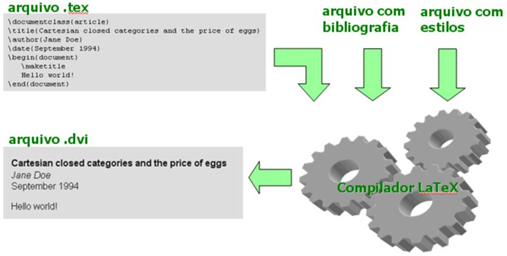
\includegraphics[scale=0.75]{Imagens/FiguraTeste.png}
% 	\textsf{\caption{Teste de uma figura em formato .png.}}
% 	\label{fig:FiguraTeste}
% \end{figure}

% \section{Operação interna e papel das expressões regulares}

% O funcionamento interno do módulo envolve a tradução de padrões \textit{RegEx}
% em operações de subgrafo sobre as estruturas moleculares representadas como
% grafos. Em termos gerais, o processo é dividido em etapas sucessivas que
% permitem converter descrições simbólicas de ligações e unidades
% monossacarídicas em estruturas compreensíveis computacionalmente.

% Primeiramente, ocorre a segmentação do padrão, na qual a expressão
% \textit{RegEx} fornecida é decomposta em módulos homogêneos, como unidades
% monossacarídicas ou ligações específicas. Por exemplo, o padrão
% \texttt{"Neu5Ac$\alpha$2-3Gal$\beta$1-4(Fuc$\alpha$1-3)GlcNAc"} é dividido em
% blocos como \texttt{"Neu5Ac$\alpha$2-3"}, \texttt{"Gal$\beta$1-4"} e
% \texttt{"Fuc$\alpha$1-3"}, representando diferentes segmentos estruturais que
% serão posteriormente analisados. Em seguida, ocorre a interpretação e expansão
% dos modificadores e quantificadores. Operadores como \texttt{+}, \texttt{*},
% \texttt{?}, intervalos \texttt{\{m,n\}} e quantificadores preguiçosos
% (\texttt{+?}) são suportados, permitindo definir repetições, ocorrências
% opcionais ou faixas de aparecimento dos motifs. Essa flexibilidade amplia a
% capacidade do módulo de reconhecer variações estruturais dentro de uma mesma
% família de glicanos. Posteriormente, aplica-se o processo de \textit{subgraph
% 	isomorphism}, em que cada segmento é buscado dentro do grafo que representa a
% estrutura glicosídica. Essa etapa utiliza algoritmos de isomorfismo de
% subgrafos para identificar correspondências exatas, mesmo em representações
% complexas que envolvem ramificações e múltiplas conexões entre unidades.

% Outro componente essencial é a implementação das operações de
% \textit{lookahead} e \textit{lookbehind}, herdadas das expressões regulares
% textuais. Elas permitem incluir ou excluir determinados contextos do padrão de
% busca sem incorporá-los ao resultado final, sendo cruciais para capturar motifs
% cuja ocorrência depende de um contexto estrutural específico.

% Por fim, ocorre a construção do caminho de correspondência, na qual um
% algoritmo iterativo reconstrói o trajeto contínuo dentro do grafo, unindo as
% correspondências parciais e validando os requisitos definidos pela expressão
% completa. Essa abordagem possibilita representar ligações específicas, como
% $\alpha$1-3 ou $\beta$1-6, bem como ambiguidade estrutural e ramificações
% expressas por meio de parênteses. Dessa forma, a notação \textit{RegEx} é
% adaptada à topologia molecular, permitindo uma modelagem altamente expressiva e
% precisa das estruturas glicosídicas.

\section{Vantagens da RegEx no contexto do \texttt{glycowork}}

Como comentado, a inovação trazida pelo \texttt{Glycan RegEx} ao framework
\texttt{glycowork} consiste na união do método tradicional de busca por motifs
com isomorfismo de subgrafo e o uso de um sistema de expressões regulares
específico para glicanos.

Sem o uso das expressões regulares, há a necessidade de uma base estática de
motifs já conhecidos - como pode ser vista no arquivo
\texttt{common\_names.json} do próprio framework -, o uso de muitas combinações
de padrões para detectar motifs complexos e específicos do glicano e a
dificuldade de capturar contextos maiores, como um motif presente apenas em um
ramo do glicano. Todos esses fatores culminam em um uso bastante rígido e, por
vezes, difícil de representar de forma computacional.

Com a introdução do sistema \texttt{Glycan RegEx} é possível escrever padrões
de buscas de motifs em um formato mais declarativo e eficaz, com uso de
operadores clássicos que permitem negação, repetição e demais operações. Dessa
forma, o algoritmo de busca de motifs tem a capacidade de gerar diversos
subgrafos intermediários (ao contrário do mecanismo anterior), encontrando a
combinação ideal de motifs de forma refinada e mais simples para o programador.

Esta camada adicional que o sistema traz pode gerar um \textit{overhead} em
estruturas mais simples do glicano quando comparado com a busca tradicional do
\texttt{glycowork} por motifs. Entretanto, quando aplicado em glicanos mais
complexos ou maiores, tal mecanismo se sobressai tanto em sua eficácia, podendo
ser mais simples escrever uma única expressão regular que atenda aos critérios,
quanto em sua eficiência.

